\documentclass[11pt]{article}
\usepackage[letterpaper,margin=1in]{geometry}
\usepackage[T1]{fontenc}
\usepackage[utf8]{inputenc}
\usepackage{graphicx}
\usepackage{booktabs}
\usepackage{array}
\usepackage{float}
\usepackage{xcolor}
\usepackage{url}
\usepackage{fancyhdr}

\graphicspath{{images/}}
\definecolor{umlblue}{RGB}{14,42,75}
\pagestyle{fancy}
\fancyhf{}
\lhead{General Inventory AI Assistant}
\rhead{COMP 5300 Final Project}
\cfoot{\thepage}
\setlength{\parindent}{0pt}
\setlength{\parskip}{0.65em}
\setlength{\headheight}{14pt}

\begin{document}

\begin{titlepage}
\centering
\vspace*{1.0in}
{\Huge\bfseries\color{umlblue} General Inventory AI Assistant\par}
\vspace{0.35in}
{\Large A Private Retrieval-Based Inventory System with Lightweight AI Intent Routing\par}
\vspace{0.8in}
\begin{tabular}{rl}
\textbf{Course:} & COMP 5300 P 1 205 Special Topics, Spring 2026 \\
\textbf{Submission:} & Final Project \\
\textbf{Student:} & Anatolie Jentimir \\
\textbf{Primary Track:} & Track D - Systems / Deployment \\
\textbf{Secondary Track:} & Track A - LLM Applications \\
\textbf{Live Demo:} & \url{https://electronicsinventory-production.up.railway.app/} \\
\textbf{AI Page:} & \url{https://electronicsinventory-production.up.railway.app/ai} \\
\end{tabular}
\vfill
{\large April 2026\par}
\end{titlepage}

\section{Introduction and Problem Framing}

This project presents \textit{General Inventory AI Assistant}, a deployed web application for managing inventory items and asking natural-language questions about the stored records. The system began as an electronics inventory app and was expanded into a general-purpose inventory manager that can support electronics, office supplies, tools, materials, books, documents, and other item types.

The practical problem is that a user may own many items stored across boxes, drawers, rooms, or project kits. Standard search requires the user to remember exact names or categories. The AI assistant reduces that friction by allowing the user to ask questions such as ``do we have paper and resistors?'', ``show all items'', ``show categories'', ``what should I restock?'', and ``what is my inventory worth?''

The success criterion is not to build the largest model, but to build a reliable deployed AI workflow that is grounded in private inventory data. A successful system should correctly route common user intents, retrieve relevant database rows, support singular and plural wording, display evidence, calculate inventory value, identify low-stock items, and avoid hallucinating items that are not present in the database.

\section{Data Statement}

The primary dataset is a private SQLite database created by the inventory application. Each row represents an item record entered by the user. The database includes fields such as category, type, model or value, quantity, unit price, location, tags, notes, and optional photo filenames.

The dataset is user-created and private. No public benchmark dataset is required for deployment because the application is intended to answer questions about the user's own inventory. At final demonstration time, the database included a small but diverse test inventory containing electronics and office-supply records. The system is designed to scale as the user adds more records.

\subsection{Licensing, Privacy, and Leakage Risks}

Because the inventory data is created by the user, there is no external dataset license requirement for the production system. However, the data can contain private details such as storage locations, prices, item photos, and project notes. For that reason, the production assistant does not require a paid external AI API. It answers from local SQLite rows and displays the retrieved evidence.

The main leakage risks are committing private database files, backups, uploaded photos, or credentials to GitHub. These files should be excluded using a \texttt{.gitignore}. Recommended exclusions include \texttt{*.db}, \texttt{*.sqlite}, \texttt{.env}, \texttt{app/uploads/}, and model checkpoint files.

\subsection{Preprocessing}

For retrieval, each inventory row is converted into a searchable text document. The preprocessing pipeline lowercases text, tokenizes words, normalizes simple singular/plural variants, and combines item fields into one retrieval representation. For example, terms such as \textit{item/items}, \textit{tool/tools}, \textit{category/categories}, \textit{sensor/sensors}, and similar variants are mapped to comparable forms.

There is no supervised train/validation/test split for the live inventory because the data changes as the user adds or edits items. Instead, evaluation uses a fixed set of manual test questions covering item lookup, multi-item lookup, category summaries, restock warnings, duplicate detection, inventory value, and no-match behavior.

\section{Baseline}

The baseline is a standard keyword search over inventory fields. This baseline is appropriate because many small inventory systems search by exact item name, category, tag, or location.

The weakness of the baseline is that it does not understand user intent. It may fail when the user asks for a command such as ``show all items'' or ``show categories'', and it may miss wording variations such as singular and plural forms. It also does not automatically run inventory-specific diagnostics such as low-stock warnings, duplicate detection, or value calculation.

\section{Method}

The final system uses a lightweight AI workflow rather than a full large language model server. This design was chosen to keep the deployed app private, fast, inexpensive, and realistic for Railway hosting.

The method contains four parts:

\begin{enumerate}
\item \textbf{Inventory row textification:} each SQLite row is converted into a searchable text document.
\item \textbf{Term normalization:} common wording variations across item names, categories, and user phrasing are normalized.
\item \textbf{Retrieval ranking:} likely matches are ranked with TF-IDF/cosine-style scoring.
\item \textbf{Intent routing:} a small trained Naive Bayes-style intent classifier routes commands such as list all, categories, restock, duplicates, and value.
\end{enumerate}

The production assistant uses retrieval-augmented generation in a local form: it retrieves database rows and generates an answer only from those rows. When no strong match exists, the system should refuse or explain that it cannot find a strong match. This reduces hallucination compared with a free-form generator.

The repository also includes optional class components: a small decoder-only Transformer prototype and a decoding/deployment lab. These files demonstrate LLM concepts such as greedy decoding, beam search, sampling, repetition penalty, KV-cache ideas, batching, quantization estimates, and model-cascade routing. They are intentionally optional so the deployed app remains lightweight.

\begin{figure}[H]
\centering
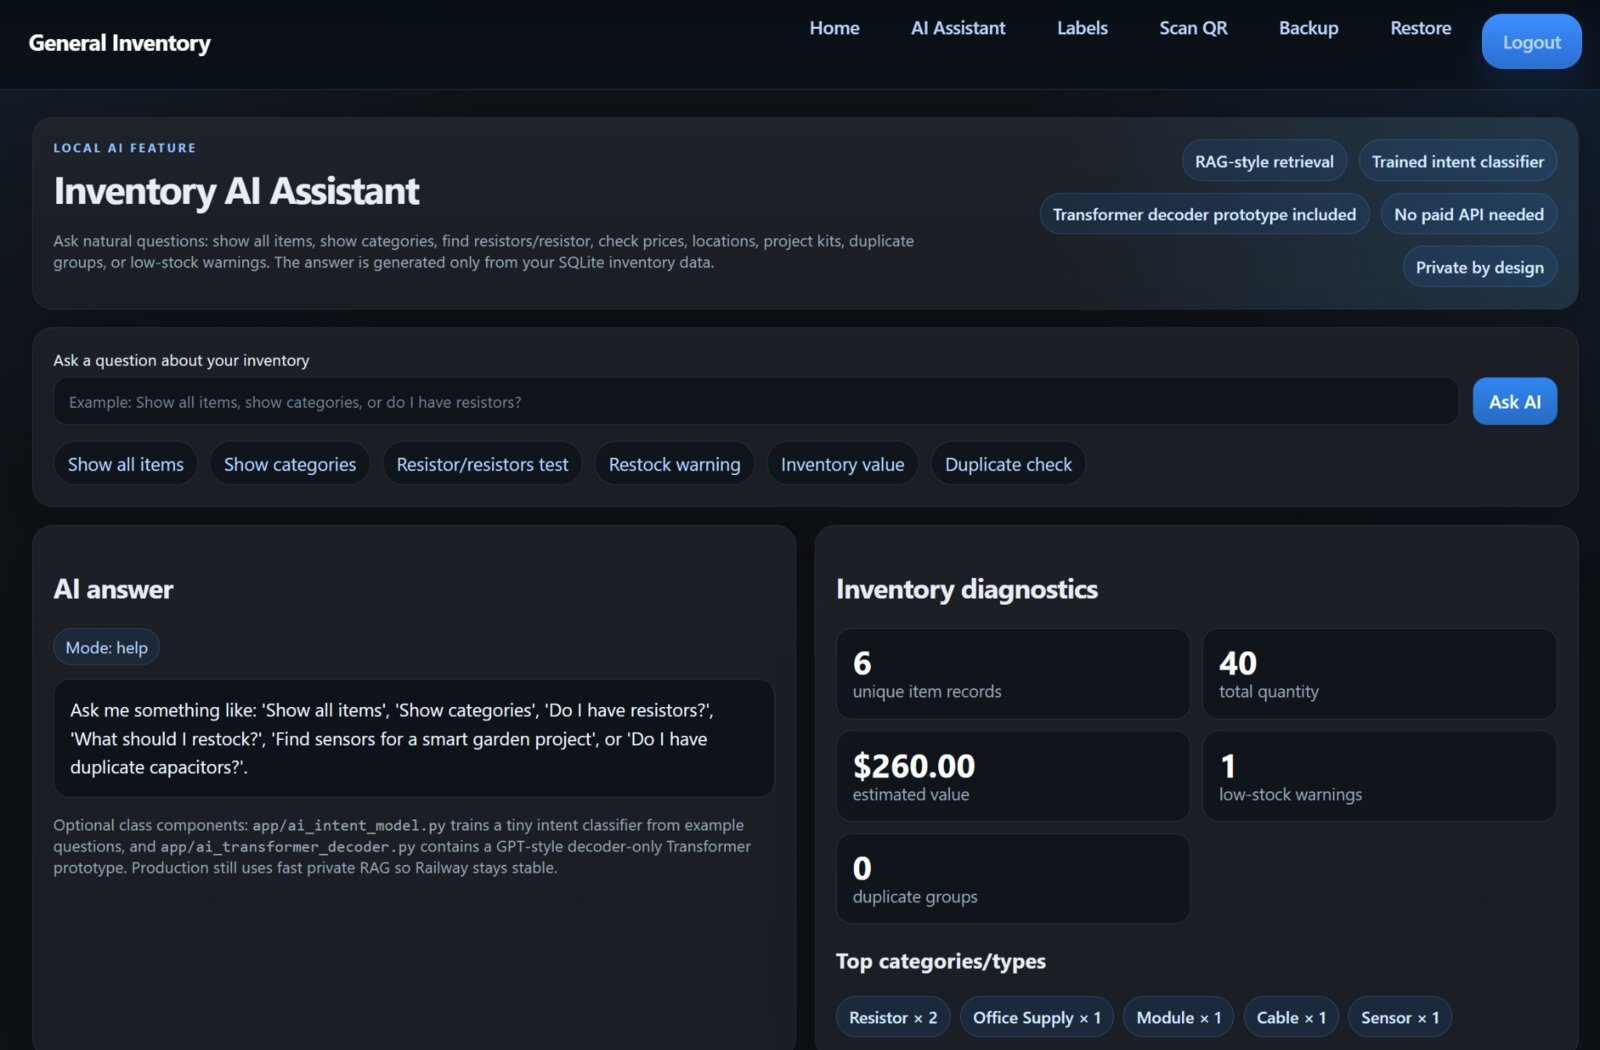
\includegraphics[width=0.95\textwidth]{ai_assistant_overview.jpg}
\caption{Deployed AI assistant interface. The system supports natural-language inventory questions, inventory diagnostics, and private retrieval over SQLite data.}
\end{figure}

\section{Training and Compute}

The production system does not require GPU training. It runs on CPU using FastAPI, SQLite, template rendering, and lightweight retrieval. The intent classifier is trained from small example phrases and runs quickly on CPU.

A full LLM server or large Transformer was deliberately not used in production. A full model would increase memory use, cold-start latency, and deployment risk. The optional Transformer decoder is kept as an offline experiment for class demonstration, while production remains retrieval-based.

\begin{table}[H]
\centering
\caption{Compute plan and deployment choices.}
\begin{tabular}{p{0.28\textwidth}p{0.62\textwidth}}
\toprule
\textbf{Component} & \textbf{Compute Choice} \\
\midrule
Production AI assistant & CPU-only retrieval and intent routing \\
Database & Local SQLite table used as the source of truth \\
External API & Not required for the production assistant \\
Optional Transformer & Offline CPU experiment; not loaded at Railway startup \\
Fallback & Use retrieval-based assistant if Transformer training is too expensive or unnecessary \\
\bottomrule
\end{tabular}
\end{table}

\begin{figure}[H]
\centering
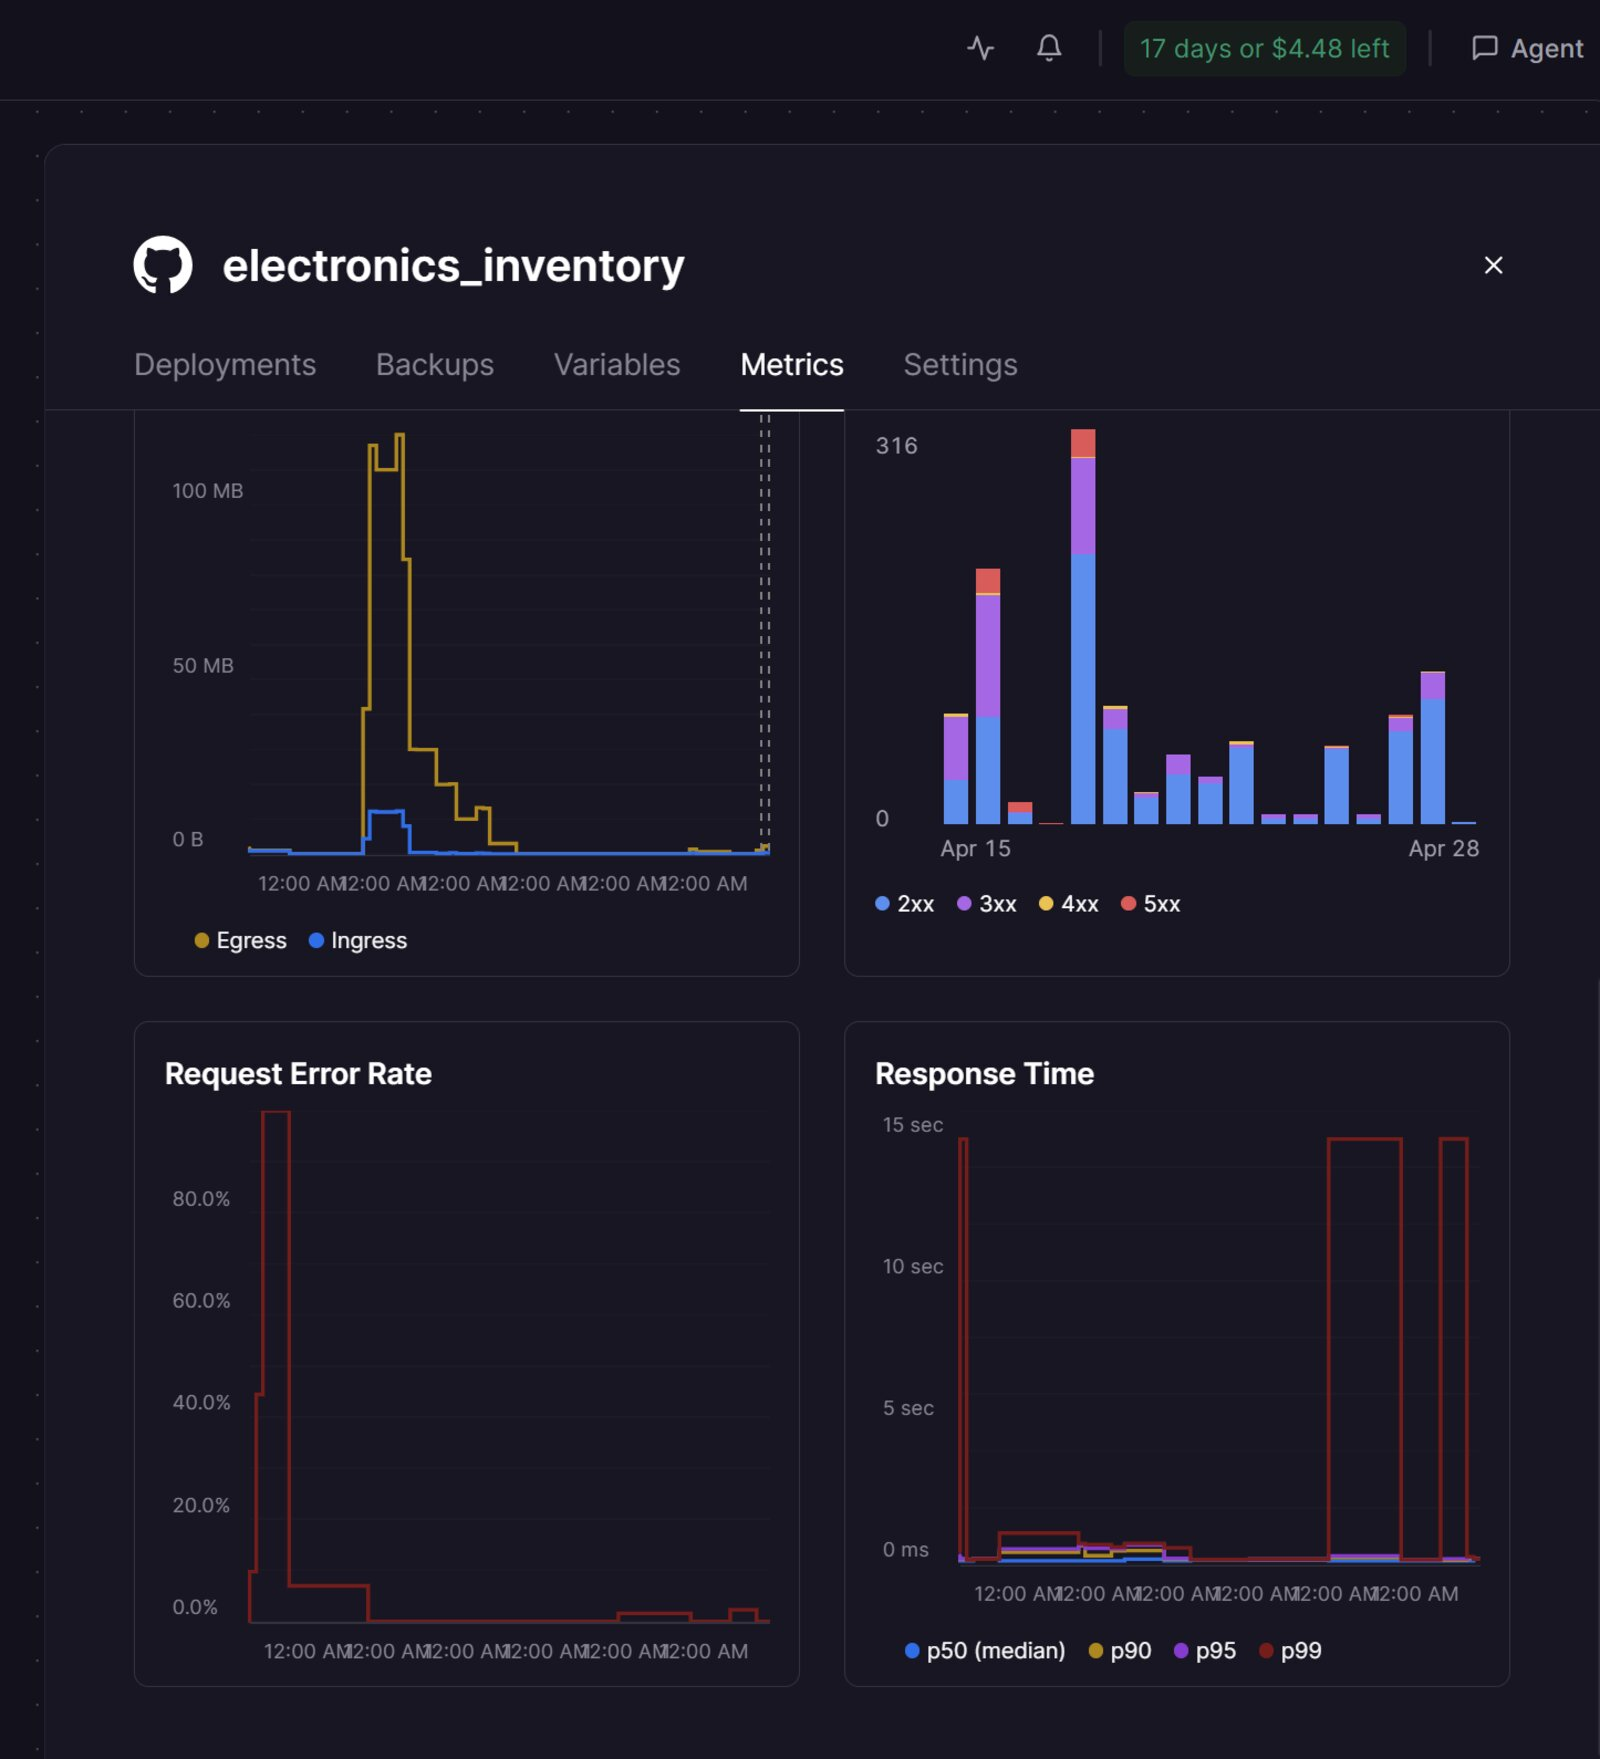
\includegraphics[width=0.95\textwidth]{railway_metrics_full.jpg}
\caption{Railway deployment metrics for the live app. CPU and memory remained small compared with a full LLM server, supporting the decision to keep production retrieval-based.}
\end{figure}

\section{Evaluation}

Evaluation focused on whether the system correctly answers practical inventory questions while remaining grounded in database rows. The main goal was not benchmark language fluency, but factual correctness, explainability, and deployment reliability.

\subsection{Primary Metrics}

The recommended metrics are:

\begin{itemize}
\item \textbf{Intent accuracy:} whether the system routes the question to the correct mode.
\item \textbf{Retrieval precision at k:} whether the expected inventory item appears in the top returned rows.
\item \textbf{No-match accuracy:} whether the assistant refuses when an item is not present.
\item \textbf{Low-stock accuracy:} whether the low-stock rule correctly identifies small quantities.
\item \textbf{Duplicate-detection correctness:} whether duplicate groups match repeated category/type/value records.
\item \textbf{Inventory value correctness:} whether the app correctly computes quantity multiplied by unit price.
\end{itemize}

\subsection{Qualitative Example}

Figure~\ref{fig:multiquery} shows a natural-language multi-item query. The user asked whether the inventory contains paper and resistors. The assistant retrieved both office-supply and electronics-related records from the same SQLite database. This demonstrates that the system works as a general inventory assistant rather than only an electronics search tool.

\begin{figure}[H]
\centering
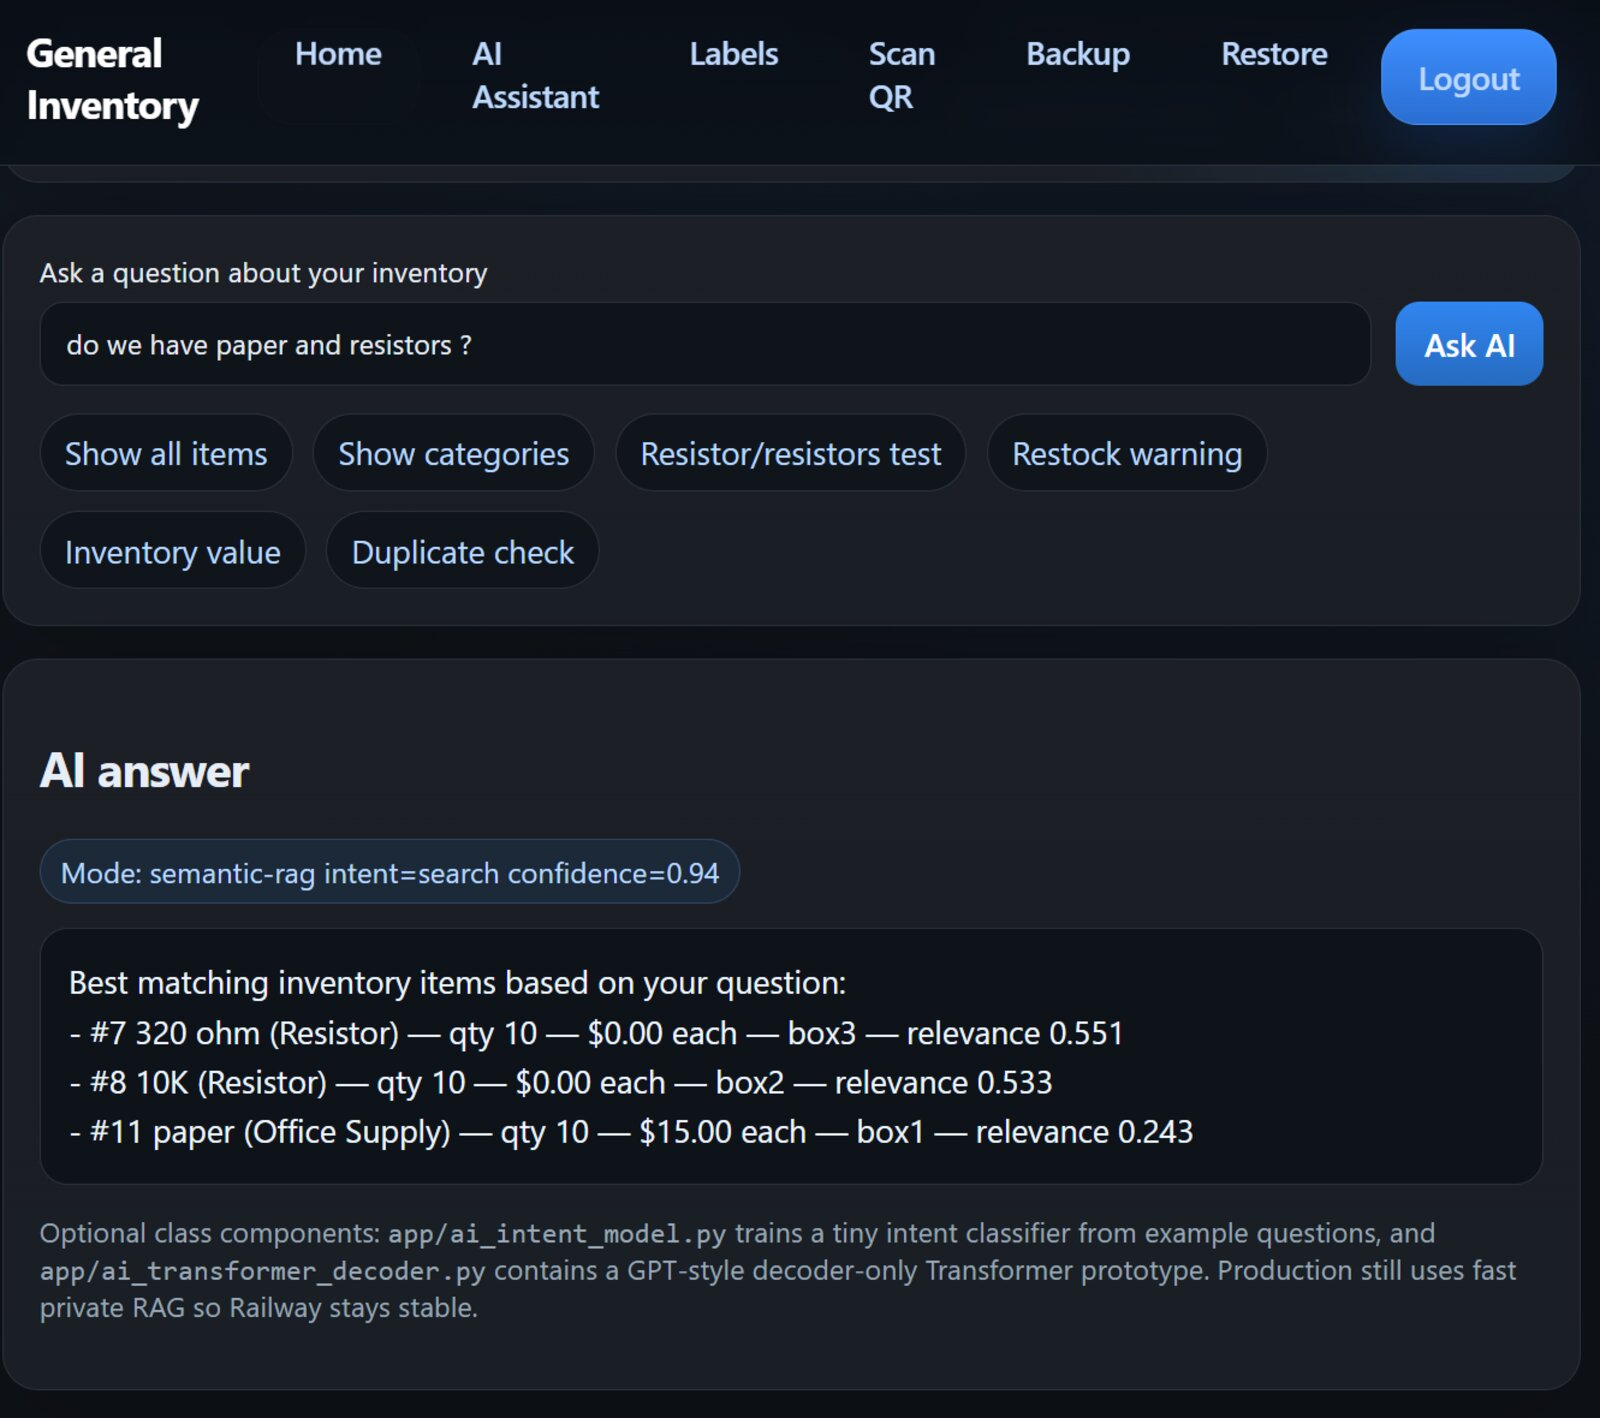
\includegraphics[width=0.95\textwidth]{qualitative_multi_item_query.jpg}
\caption{Qualitative evaluation example: a multi-item natural-language query retrieves both paper and resistor records with quantities, prices, locations, and relevance scores.}
\label{fig:multiquery}
\end{figure}

\subsection{Diagnostic Analysis and Ablations}

Diagnostic tests included commands for showing all items, showing categories, querying a single item, querying multiple items, checking low stock, checking duplicates, calculating total value, and asking for an item that does not exist. The system performed best when item records included clear names, categories, and locations.

Ablation-style comparisons were used to reason about design choices. Exact keyword search is simple, but weaker for wording variations and special commands. Adding normalization improves matches across common phrasing differences. Adding intent routing improves command-style questions such as ``show all items'', ``show categories'', and ``inventory value''. The optional decoder prototype is useful for learning and experimentation, but retrieval is safer for factual inventory answers because it stays grounded in database rows.

\section{Responsible AI}

The main responsible-AI concern is privacy. Inventory records can reveal private possessions, storage locations, costs, and project details. The deployed assistant avoids sending this data to a paid external AI service. It uses the local database as context and shows retrieved evidence so the user can verify the answer.

The second concern is hallucination. A general language model may invent items. This system mitigates that risk by grounding answers in retrieved SQLite rows and displaying evidence. If the database does not contain a strong match, the assistant should not fabricate one.

The third concern is robustness. The system can still fail on very misspelled or vague queries, inconsistent item names, or missing prices. Missing prices are treated as zero-dollar values until the user edits the record. Future improvements should include stronger fuzzy matching, synonym dictionaries, and more formal test sets.

\section{Limitations}

The final application is not a full LLM chatbot. It is a lightweight AI inventory assistant optimized for deployment, privacy, and correctness. It depends on the quality of user-entered item names, categories, tags, and notes. If the inventory records are vague, retrieval quality will decrease.

The optional Transformer decoder is intentionally small and is not expected to outperform retrieval on factual inventory questions. It exists to demonstrate large-model architecture concepts for the course while keeping production stable.

\section{Conclusion and Next Steps}

The final system is a deployed general inventory web app with a private AI assistant. It supports natural-language inventory search, category summaries, low-stock warnings, duplicate checks, inventory value calculation, plural/wording normalization, and evidence-based answers.

The main lesson is that a small grounded AI workflow can be more practical than a large model for private inventory management. Retrieval and intent routing are sufficient for many real user questions, while a large Transformer can remain optional for experimentation.

Future work includes fuzzy spelling correction, barcode support, CSV import/export, stronger duplicate detection, more charts, voice input, larger evaluation sets, and a formal model-card or datasheet for deployment documentation.

\end{document}
